\documentclass[a4paper,12pt]{book}

% Paquetes necesarios
\usepackage[utf8]{inputenc}   % Codificación de caracteres
\usepackage[spanish]{babel}   % Idioma español
\usepackage[T1]{fontenc}      % Codificación de fuentes
\usepackage{amsmath, amssymb} % Símbolos matemáticos
\usepackage{graphicx}         % Inclusión de gráficos
\usepackage{cite}             % Gestión de citas
\usepackage{hyperref}         % Enlaces y referencias
\usepackage{geometry}         % Configuración de márgenes
\usepackage{fancyhdr}         % Encabezados y pies de página
\usepackage{titlesec}         % Formato de títulos
\usepackage{booktabs}         % Tablas profesionales
\usepackage{caption}          % Personalización de leyendas
\usepackage{enumitem}         % Personalización de listas
\usepackage{float}
\usepackage{tcolorbox}
\usepackage[table]{xcolor} % Paquete para colores en tablas
\usepackage{colortbl}       % Complemento para colorear celdas específicas
\usepackage{multirow}       % Combinar celdas en tablas
\usepackage{makecell}       % Combinar celdas en tablas
\usepackage{enumitem}
\usepackage{amsmath}
\usepackage{eurosym}
\usepackage{tikz}
\usepackage{listings}
\usepackage{color}
\usepackage{float}
\usepackage{pdfpages}

% Configuración de márgenes
\geometry{left=3cm, right=3cm, top=2.5cm, bottom=2.5cm}

% Configuración de encabezados y pies de página
% \setlength{\headheight}{14.49998pt}
\pagestyle{fancy}
\fancyhf{}
<<<<<<< HEAD
\fancyhead[L]{Universidad de Granada}
\fancyhead[L]{\nouppercase{\chaptername~\thechapter. \leftmark}}

% \fancyhead[C]{Escuela Técnica Superior de Ingenierías Informática}
=======
%\fancyhead[L]{Universidad de Granada}
\fancyhead[L]{\nouppercase{\chaptername \thechapter. \leftmark}}
>>>>>>> 6880c38 (añadiendo el formato adecuado de los libros que tengo)
\fancyhead[R]{Inteligencia Artificial}
\fancyfoot[L]{\rule[0pt]{\textwidth}{0.2pt}\\Ismael Sallami Moreno}
\fancyfoot[C]{\rule[0pt]{\textwidth}{0.2pt}\\\thepage}
\fancyfoot[R]{\rule[0pt]{\textwidth}{0.2pt}\\\today}
<<<<<<< HEAD
=======

>>>>>>> 6880c38 (añadiendo el formato adecuado de los libros que tengo)
\renewcommand{\sectionmark}[1]{\markboth{#1}{}} % Configura \leftmark para que solo muestre la sección


% Formato de títulos
\titleformat{\section}{\large\bfseries}{\thesection.}{0.5em}{}
\titleformat{\subsection}{\normalsize\bfseries}{\thesubsection.}{0.5em}{}

% Datos del documento
\title{\textbf{Temario Inteligencia Artificial}}
\author{
    Ismael Sallami Moreno \\
    \texttt{ism350zsallami@correo.ugr.es}
}
\date{
    \vspace{1cm}
    \begin{tabular}{rl}
        \textbf{Asignatura:} & Inteligencia Artificial \\
        \textbf{Tema:} & Temario \\
        \textbf{Fecha:} & \today
    \end{tabular}
}

\begin{document}

% Portada
\begin{titlepage}
    \begin{center}
        % \vspace*{1cm}
        
        % \Huge
        % \textbf{Práctica Contabilidad Financiera II}
        \Huge \textbf{Temario Inteligencia Artificial} 
        % \vspace{0.5cm}
        % \LARGE
        % \textbf{Ismael Sallami Moreno}\\
        % \LARGE
        % \texttt{ism350zsallami@correo.ugr.es}
        % \LARGE
        % \url{https://github.com/Ismael-Sallami}
        
        % \vfill
        
        % \Large
        % \textbf{Universidad de Granada}
        
        \vspace{0.8cm}
        
        \begin{tikzpicture}[remember picture, overlay]
            \node[opacity=0.2] at (current page.center) {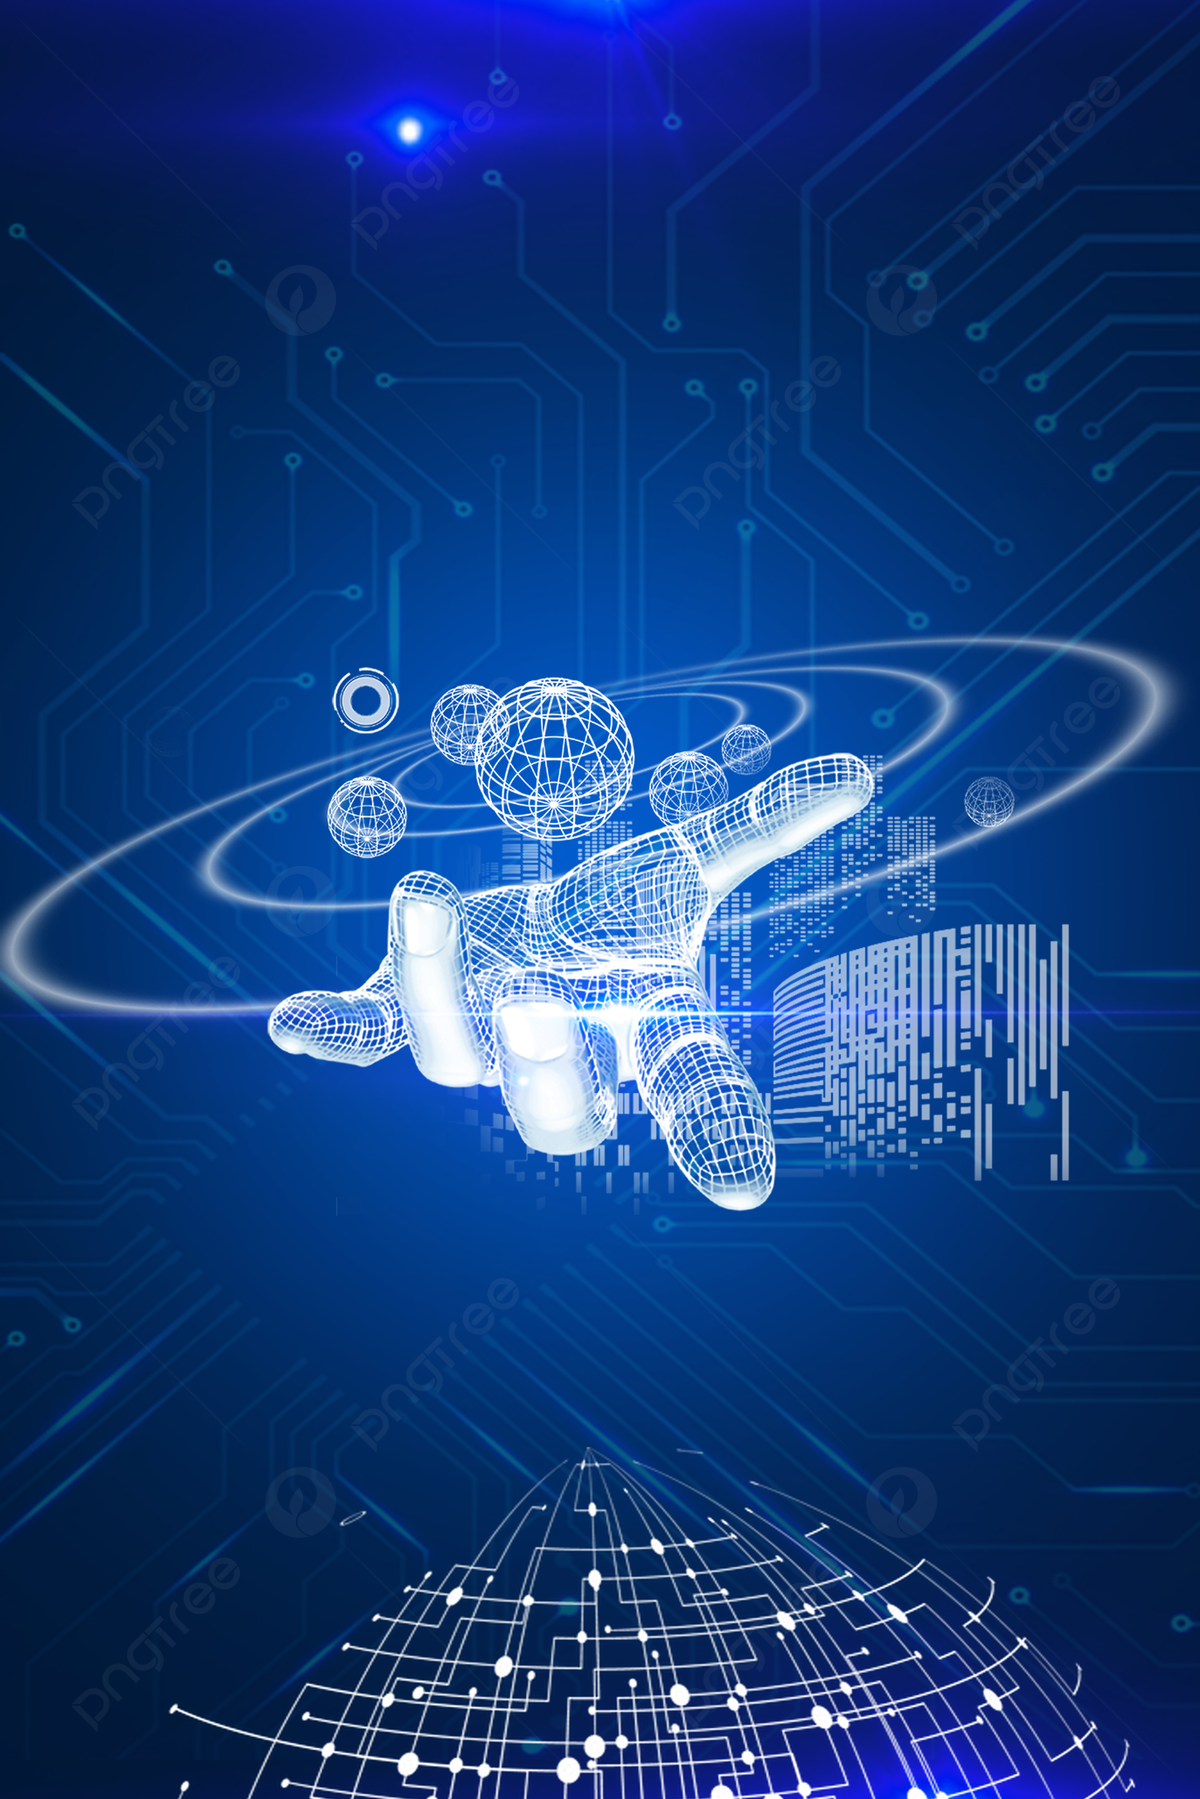
\includegraphics[width=\paperwidth,height=\paperheight]{portada.png}};
            \node[align=center] at (current page.center) {
                
                \vspace{0.5cm}
                \LARGE \textbf{Ismael Sallami Moreno} \\
                \LARGE \texttt{ism350zsallami@correo.ugr.es} \\
                \LARGE \url{https://ismael-sallami.github.io/} \\
                \LARGE \url{https://elblogdeismael.github.io/} \\
                \vspace{2cm}
                \Large \textbf{Universidad de Granada} \\
                \vspace{0.8cm}
                % \Large \textbf{2025}
            };
        \end{tikzpicture}
        \vfill
        
        \Large
        \textbf{2025}
        
    \end{center}
\end{titlepage}
\newpage


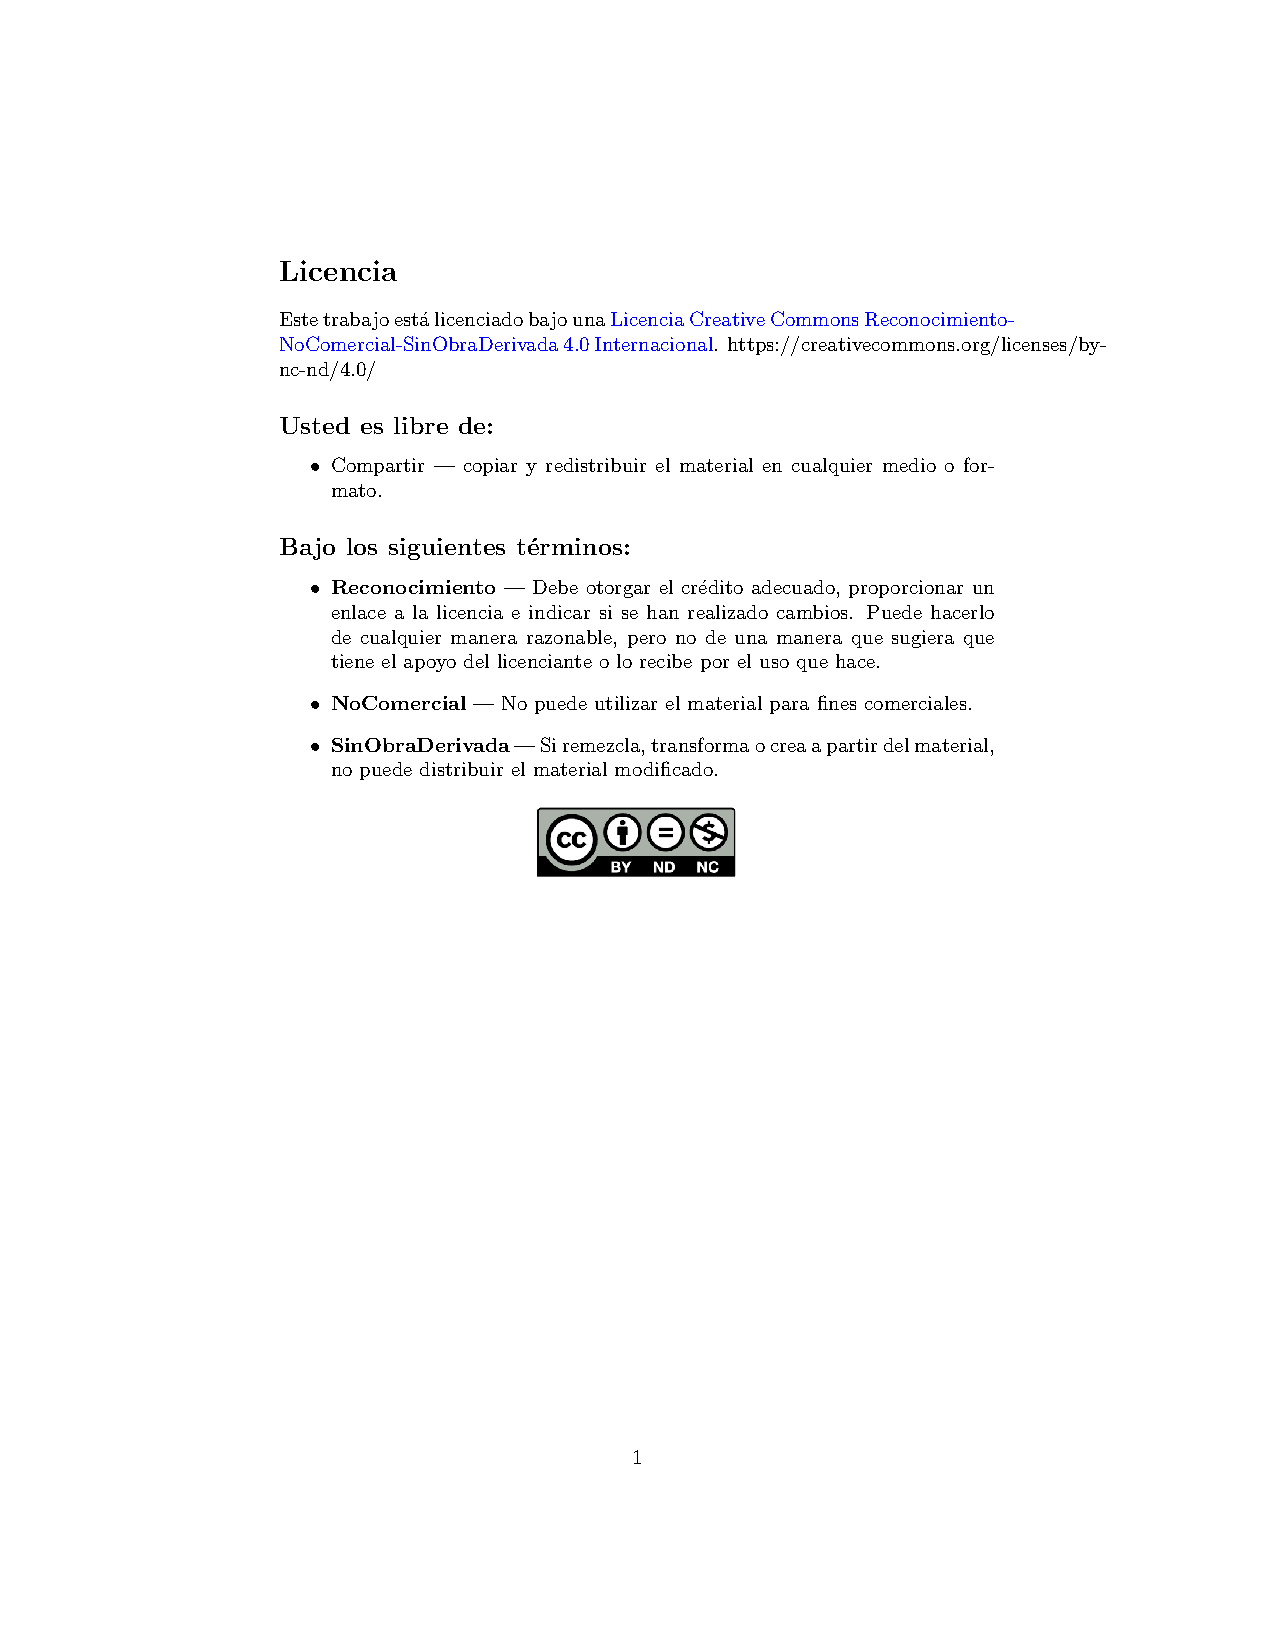
\includepdf[pages=-]{../../../../licencia.pdf}

% Tabla de contenidos
\tableofcontents
\newpage

\chapter{Introducción}
\section{Apuntes de CLase}
\section{Introducción: Inteligente}
Debemos de definir la inteligencia artificial
usando la palabra inteligente, la cual es difícil de definir. Se dan diferentes definiciones de Harvard y otras universidades/entidades reconocidas. 

\section{Definición de IA}

Podemos tener varias definiciones de IA, como pueden ser sistemas que actúan/piensan como humanos, o bien sistemas que actúan/piensas racionalmente. Una de ellas puede ser: "Campo de estudio que busca explicar y emular el comportamiento inteligente en términos de procesos computacionales"

Un ejemplo de IA que menciona el profesor reiteradamente es el caso de los \textit{cajeros automáticos}.

\begin{tcolorbox}[colback=blue!20, colframe=blue]
Se garantiza que una pregunta sobre las definiciones de IA cae.
    
\end{tcolorbox}

Asociamos el concepto de IA a racional debido a que se quiere desarrollar con la capacidad de poder tomar decisiones como los humanos.

Hay distintos softwares en los dispositivos que podemos relacionarlos con la acción de que \textit{piensan} debido a que usan inteligencia artifical, como es el caso de programas de ajedrez. ¿Es esto correcto? No podemos afirmar esto exactamente, ya que según autores pensar es emular la mente humana, cosa que no es capaz de hacer la IA debido a que solo esta entrenado a hacer las mejores jugadas para ganarte, mientras que tu puedes pensar sobre otras temáticas y tener cierto \textit{pensamiento libre}.

Si afirmamos que piensan como humanos, debemos de tener en cuenta el \textit{pensamiento cognitivo}.

La IA según el libro del \textit{Porque} (recibió el premio Turing), tiene 3 niveles:
\begin{enumerate}
    \item Aprendizaje automático.
    \item Simular al humano.
    \item Capacidad de imaginar, lo cual, a día de hoy es inalcanzable.
\end{enumerate}

En cuanto a la creatividad, hay cierta\textit{ creatividad cognitiva }en temas específicos.

El llamado 'no alineamiento con los humanos' es lo que ocurre cuando una IA no tiene información sobre ese tema o bien no esta entrenado, pues en este caso se lo inventa.

El Test de Turing, es aquel en el que si una IA consigue pasar desapercibido como humano, pues efectivamente pasa este Test.

En esta asignatura vamos a seguir la Teoría del Agente, que es la idea más aceptada hoy día y más usada. Este percibe el entorno y actúa de una manera específica. 

Se usa la palabra \textit{racional} aludiendo a inteligente.

Un agente racional actúa de manera correcta según la información que posee.

El origen del término de IA recae en John McCarthy. Los pioneros de la IA son varios, entre los que podemos encontrar a Alan Turing, Marvin Minsky,...

En el debate de la IA se menciona una IA fuerte y una débil, que son sistemas que actúan como humanos y racionalmente vs las que piensan como IA.

En cuanto al recorrido de la IA a lo largo de la historia, podemos destacar distintas épocas como es la Edad de Oro, Invierno de IA,...

Von Neumann propone el algoritmo MiniMax, el que afirma que el juego es una situación conflictiva en la que tomamos decisiones sabiendo que los demás también las toman, determinando el resultado en base a las decisiones realizadas.
Un hecho histórico destacable, es que Napoleón murió pensando que había perdido jugando al ajedrez pensando que perdió frente al primer sistema inteligente, aunque puede que haya sido un humano. 
Otro de los avances importantes es el caso de los cohes autónomos.

En cuanto a los tipos de IA podemos mencionar:

\begin{itemize}
    \item IA débil: una máquina que compite con un humano en una actividad específica.
    \item IA fuerte: IA que aplica inteligencia para cualquier problema.
    \item IA general: alcanza el nivel cognitivo humano.
    \item Super-IA: capacidad que es mucho mayor que cualquier cerebro humano en cualquier campo.
\end{itemize}

\chapter{Agentes}
\section{Apuntes de CLase}
\section{Concepto}
La Teoría de Agentes(denotado a continuación como \textbf{TA}) es un sistema de ordenador, situado en un entorno, capaz de realizar acciones de manera autónoma y que es flexible en base a las situaciones que se le presentan.

\section{Agentes Inteligentes}

Desarrolla un enfoque basado en agentes y lleva a cabo percepciones procesada mediante algoritmos de análisis y toma de decisiones. 
La TA se usa actualmente en la mayoría de ámbitos y es lo que más se usa hoy en día.

En cuanto a los tipos de agentes encontramos:

\begin{itemize}
    \item Reactivo: reacciona en base al entorno.
    \item Pro-activo: no solo actúan en respuesta al entorno, sino que puedan analizar acciones a llevar a cabo.
    \item  Social: son además capaces de interactuar.
    \item Multiagente: esta implementado como varios agentes interactuando.
\end{itemize}

La interacción entre agentes se lleva a cabo mediante: cooperación, coordinación y la negociación.


\section{Arquitecturas de Agentes}

Podemos distinguir entre:

\begin{itemize}
    \item Reactivo: reacciona en base a la situación en la que se encuentra, eligiendo la más adecuada en base a lo que sabe.
    \item Deliberativo: toma decisiones basadas en razonamiento, planificación y modelos internos del mundo.
\end{itemize}

\chapter{Búsqueda en Espacios de Estados}
\section{Apuntes de CLase}
\subsection{Diseño de un agente deliberativo: búsqueda en espacios de estados}

El agente dispone de un modelo del mundo donde actúa, modelo de efectos de las acciones sobre el mundo, es capaz de razonar sobre esos modelos para decidir que hacer para conseguir un objetivo.


Tras esta introducción, vamos a pasar a ver el espacio de estados.

\textbf{Espacio de Estados: } Representación del
conocimiento a través de las acciones del
agente.

\textbf{Búsqueda en Espacios de Estados: } Resolución del problema mediante proyección
de las distintas acciones.

Como ejemplo de agente deliberativo, se trata \textit{el problema del viajante de comercio}.



\newpage
% Referencias
\begin{thebibliography}{99}
\bibitem{Referencia1}
Ismael Sallami Moreno, \textbf{Estudiante del Doble Grado en Ingeniería Informática + ADE}, Universidad de Granada, 2025.
% \bibitem{Referencia2}
% Autor(es), \emph{Título del libro}, Editorial, año.

% \bibitem{Referencia3}
% Autor(es), \emph{Título del documento}, Nombre de la Conferencia, páginas, año.
\end{thebibliography}

\end{document}
